%%%%%%%%%%%%%%%%%%%%%%%%%%%%%%%%%%%%%%%%%
% Masters/Doctoral Thesis 
% LaTeX Template
% Version 1.43 (17/5/14)
%
% This template has been downloaded from:
% http://www.LaTeXTemplates.com
%
% Original authors:
% Steven Gunn 
% http://users.ecs.soton.ac.uk/srg/softwaretools/document/templates/
% and
% Sunil Patel
% http://www.sunilpatel.co.uk/thesis-template/
%
% License:
% CC BY-NC-SA 3.0 (http://creativecommons.org/licenses/by-nc-sa/3.0/)
%
% Note:
% Make sure to edit document variables in the Thesis.cls file
%
%%%%%%%%%%%%%%%%%%%%%%%%%%%%%%%%%%%%%%%%%


% -----------------------
% --- Document config ---
% -----------------------

% default font size, one-sided printing (no margin offsets)
\documentclass[11pt, oneside]{Thesis}

\graphicspath{{Pictures/}} % directory of pictures

\usepackage[square, numbers, comma, sort&compress]{natbib} 
\usepackage{amsmath}
%\usepackage{amssymb}
\usepackage{graphicx}
\usepackage{graphbox}
%\usepackage{indentfirst}
%\usepackage{setspace}
%\doublespacing
%\usepackage{cite}
%\usepackage{hyperref}
%\usepackage{float}
\usepackage{notoccite}
%\usepackage{epstopdf}
\usepackage{caption}
\usepackage{subcaption}
\usepackage{tabu}
\usepackage{multirow}
\usepackage{longtable}
\usepackage{array}
\usepackage{pifont}
\usepackage{hhline}
\usepackage{textcomp}
%\usepackage{gensymb}
\usepackage{breqn}
\usepackage{rotating}
\usepackage{float}
\usepackage{tikz}
\usepackage{minibox}
\usepackage[autostyle]{csquotes}
\usepackage[load-configurations = abbreviations]{siunitx}
\usetikzlibrary {shadows}
\usetikzlibrary{automata, positioning, arrows, calc}
\usetikzlibrary{arrows}
\usepackage{xurl}

\title{\ttitle} % Defines the thesis title - don't touch this

\usepackage[T1]{fontenc}
\usepackage{helvet}

\begin{document}
	%TODO comments are way to much here...
\tikzset{
	->, % makes the edges directed
	>=stealth', % makes the arrow heads bold
	node distance=3cm, % specifies the minimum distance between two nodes. Change if necessary.
	every state/.style={thick, fill=gray!10}, % sets the properties for each ’state’ node
	initial text=$ $, % sets the text that appears on the start arrow
}

\setstretch{1.5} % Line spacing of 1.3

% PDF meta-data
\hypersetup{pdftitle={\ttitle}}
\hypersetup{pdfauthor=\authorname}

\frontmatter
% Cover
\thispagestyle{empty} % No headers or page numbers

\begin{center}
	\begin{figure}
		\begin{center}
			
\includegraphics[height=4cm]{TU-Berlin-Logo}
		\end{center}
	\end{figure}
	\small
	\textbf{TECHNISCHE  UNIVERSITÄT BERLIN\\
		FAKULTÄT ELEKTROTECHNIK UND INFORMATIK\\
		FACHGEBIET LICHTTECHNIK}
	
	\vfill
	\Large
	\textbf{{\ttitle}} \\ 
	
	\vfill
	\small
	Bachelor of Science  in technischer Informatik  \\
	(Energie- und Automatisierungstechnikt)\\
	\vspace*{0.5cm}
	
	\vfill
	\small
	von\\
	\large
	\textbf{Name:} {\authornames}\\
	\textbf{E-Mail:} conrad.klaus@campus.tu-berlin.de\\
	\textbf{Matrikelnummer:} 401498 \\
	
	\small
	
	\vfill
	\small
	Betreut von\\
	\normalsize
	\textbf{Prof. Dr.-Ing. Stephan Völker\\
		Frithjof Barkholdt, M.Sc.}
	
	\vfill
	\small
	Berlin, 2022\\
	
\end{center}


% Statement
%-----------------------------------------
% Statement(manually formatted)
%-----------------------------------------
\thispagestyle{plain} % No headers

{\huge\textbf{Erklärung der Urheberschaft}}
\vspace{1cm}


\Large

Ich erkläre hiermit an Eides statt, dass ich die vorliegende Arbeit "\ttitle" ohne Hilfe
Dritter und ohne Benutzung anderer als der angegebenen Hilfsmittel angefertigt habe;
die aus fremden Quellen direkt oder indirekt übernommenen Gedanken sind als solche
kenntlich gemacht.
Die Arbeit wurde bisher in gleicher oder ähnlicher Form in keiner
anderen Prüfungsbehörde vorgelegt.


\vspace{1cm}
\begin{flushright}
\begin{tabular}{@{} c@{} c}
	\vspace*{-1.5em} \hspace*{1em}
	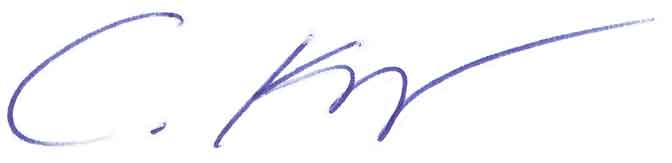
\includegraphics[width=6cm]{Pictures/Signature}&\\
	\makebox[8cm]{\dotfill} &, Berlin, \submissionDate\\
	(\authorname) & 
\end{tabular}
\end{flushright}
\newpage


% Abstract
\thispagestyle{plain} % No headers

{\huge\textbf{Abstract}}
\vspace{1cm}

Lorem Ipsum is simply dummy text of the printing and typesetting industry. Lorem Ipsum has been the industry's standard dummy text ever since the 1500s, when an unknown printer took a galley of type and scrambled it to make a type specimen book. It has survived not only five centuries, but also the leap into electronic typesetting, remaining essentially unchanged. It was popularised in the 1960s with the release of Letraset sheets containing Lorem Ipsum passages, and more recently with desktop publishing software like Aldus PageMaker including versions of Lorem Ipsum.





% List of contents, figures, table pages
\cleardoublepage
\tableofcontents


\mainmatter	% Begin numeric (1,2,3...) page numbering
\pagestyle{fancy} % The page style headers have been "empty" all this time, now use the "fancy" headers as defined before to bring them back

% Chapter Template

\chapter{Chapter Title Here} % Main chapter title

\label{ChapterX} % Change X to a consecutive number; for referencing this chapter elsewhere, use \ref{ChapterX}

\lhead{Chapter X. \emph{Chapter Title Here}} % Change X to a consecutive number; this is for the header on each page - perhaps a shortened title

%----------------------------------------------------------------------------------------
%	SECTION 1
%----------------------------------------------------------------------------------------

\section{Main Section 1}

Lorem ipsum dolor sit amet, consectetur adipiscing elit. Aliquam ultricies lacinia euismod. Nam tempus risus in dolor rhoncus in interdum enim tincidunt. Donec vel nunc neque. In condimentum ullamcorper quam non consequat. Fusce sagittis tempor feugiat. Fusce magna erat, molestie eu convallis ut, tempus sed arcu. Quisque molestie, ante a tincidunt ullamcorper, sapien enim dignissim lacus, in semper nibh erat lobortis purus. Integer dapibus ligula ac risus convallis pellentesque.

\citep{Reference2, Reference1, Reference3}

%-----------------------------------
%	SUBSECTION 1
%-----------------------------------
\subsection{Subsection 1}

Nunc posuere quam at lectus tristique eu ultrices augue venenatis. Vestibulum ante ipsum primis in faucibus orci luctus et ultrices posuere cubilia Curae; Aliquam erat volutpat. Vivamus sodales tortor eget quam adipiscing in vulputate ante ullamcorper. Sed eros ante, lacinia et sollicitudin et, aliquam sit amet augue. In hac habitasse platea dictumst.

%-----------------------------------
%	SUBSECTION 2
%-----------------------------------

\subsection{Subsection 2}
Morbi rutrum odio eget arcu adipiscing sodales. Aenean et purus a est pulvinar pellentesque. Cras in elit neque, quis varius elit. Phasellus fringilla, nibh eu tempus venenatis, dolor elit posuere quam, quis adipiscing urna leo nec orci. Sed nec nulla auctor odio aliquet consequat. Ut nec nulla in ante ullamcorper aliquam at sed dolor. Phasellus fermentum magna in augue gravida cursus. Cras sed pretium lorem. Pellentesque eget ornare odio. Proin accumsan, massa viverra cursus pharetra, ipsum nisi lobortis velit, a malesuada dolor lorem eu neque.

%----------------------------------------------------------------------------------------
%	SECTION 2
%----------------------------------------------------------------------------------------

\section{Main Section 2}

Sed ullamcorper quam eu nisl interdum at interdum enim egestas. Aliquam placerat justo sed lectus lobortis ut porta nisl porttitor. Vestibulum mi dolor, lacinia molestie gravida at, tempus vitae ligula. Donec eget quam sapien, in viverra eros. Donec pellentesque justo a massa fringilla non vestibulum metus vestibulum. Vestibulum in orci quis felis tempor lacinia. Vivamus ornare ultrices facilisis. Ut hendrerit volutpat vulputate. Morbi condimentum venenatis augue, id porta ipsum vulputate in. Curabitur luctus tempus justo. Vestibulum risus lectus, adipiscing nec condimentum quis, condimentum nec nisl. Aliquam dictum sagittis velit sed iaculis. Morbi tristique augue sit amet nulla pulvinar id facilisis ligula mollis. Nam elit libero, tincidunt ut aliquam at, molestie in quam. Aenean rhoncus vehicula hendrerit.


\cleardoublepage
\addtotoc{Abbildungsverzeichnis}
\listoffigures % Write out the List of Figures
\lhead{\emph{Abbildungsverzeichnis}}

\cleardoublepage
\addtotoc{Tabellenverzeichnis}
\listoftables % Write out the List of Tables
\lhead{\emph{Tabellenverzeichnis}}


% --------------------
% --- Bibliography ---
% --------------------
\cleardoublepage
\label{Literaturverzeichnis}
\addtotoc{Literaturverzeichnis}
\lhead{\emph{Literaturverzeichnis}} % Change the page header to say "Bibliography"

\bibliographystyle{unsrtnat} % Use the "unsrtnat" BibTeX style for formatting the Bibliography

\bibliography{Bibliography} % The references (bibliography) information are stored in the file named "Bibliography.bib"



\end{document}  